\section{Representative Model Grid}\label{sec:grid}

\subsection{Grid computation}

We compute a stellar model grid as the training dataset. We aim to cover stars with approximate solar mass on the main-sequence and the subgiant phases. We consider four independent fundamental inputs which are stellar mass ($M$), initial helium fraction ($Y_{\rm init}$), initial metallicity ([Fe/H]$_{\rm init}$), and the mixing-length parameter ($\alpha_{\rm MLT}$). 
%
We calculated three model dataset for different purposes. The primary dataset is a standard model grid with uniform mass step. This model grid is used for all preliminary tests and also for the final training. 
%
We also calculate an additional dataset to increase the grid resolution for $M$ > 1.05$\rm M_{\odot}$. Because we find that the blue hook feature (where global parameters sharply vary) is relatively hard to train. This dataset is only used in the final training. 
Details of parameter ranges and steps of the two grids are listed in Table \ref{tab:grid}. 
%
For validating and testing GP predictions, we computed off-grid models with randomly sampled fundamental inputs as a third dataset. 
%
%4,880 tracks with input parameters that are randomly sampled in the grid ranges for validating GPR models. The evolution time step was mainly controlled by the set-up tolerances on changes in surface effective temperature and luminosity. We also saved structural models for computing theoretical oscillation models.
%
The computation of evolutionary tracks starts at the Hayashi line with pre-main-sequence central temperature at 300,000K and terminates at the base of red-giant branch (RGB) where $\log g$ = 3.6dex. Note that we only use models after the zero-age-main-sequence (ZAMS), which is defined as the point where core-hydrogen burning contributes over 99.9\% of the total luminosity. 
%

\begin{table}
	\centering
	\caption{Computation of Stellar model grid.}
	\label{tab:grid}
	\begin{tabular}{llll} % four columns, alignment for each
		\hline
		\multicolumn{3}{c}{Primary dataset}\\
		\hline
		Input Parameter & Range & Increment \\
        \hline
	$M$ ($\rm M_{\odot}$) & 0.80 -- 1.20 &  0.01\\
        $\rm{[Fe/H]}$ (dex) & -0.5 -- 0.2/0.2 -- 0.5 & 0.1/0.05\\
        	$Y_{\rm init}$ & 0.24 -- 0.32 & 0.02\\
        $\alpha_{\rm{MLT}}$  & 1.7 -- 2.5&  0.2\\
        \hline
       \multicolumn{3}{c}{Additional dataset}\\
	\hline
	Input Parameter & Range & Increment \\
        \hline
	$M$ ($\rm M_{\odot}$)  & 1.055 -- 1.195 &  0.01\\
        $\rm{[Fe/H]}$ (dex) & 0.25 -- 0.45 & 0.1\\
        	$Y_{\rm init}$ & 0.25 -- 0.31 & 0.02\\
        $\alpha_{\rm{MLT}}$  & 1.8-- 2.4&  0.2\\
 %       \hline
 %       \multicolumn{3}{c}{Off-grid dataset}\\
%        \hline
%        \multicolumn{3}{c}{Input Parameters} &N\\
%       \hline
%        Randomly sampled 
%         \multicolumn{3}{l}{Random $M$, [Fe/H]$_{\rm init}$ = 0.0, $Y_{\rm init}$ = 0.28, $\alpha_{\rm MLT}$ = 2.1 } & 44\\
%        \multicolumn{3}{l}{Random $M$ and [Fe/H]$_{\rm init}$, $Y_{\rm init}$ = 0.28, $\alpha_{\rm MLT}$ = 2.1 }&174\\
%        \multicolumn{3}{l}{Random $M$, [Fe/H]$_{\rm init}$, $Y_{\rm init}$, and $\alpha_{\rm MLT}$}&4880\\
	\hline
	\end{tabular}
\end{table}

\subsection{Input physics}\label{subsec:stellar_model}

We use the stellar code Modules for Experiments in Stellar Astrophysics
(\textsc{MESA}, version 12115) to construct stellar grids. 
\textsc{MESA} is an open-source stellar evolution package which is undergoing active development. 
Descriptions of input physics and numerical methods
can be found in \citet{2011ApJS..192....3P,2013ApJS..208....4P, 2015ApJS..220...15P}.
We adopted the solar chemical mixture [$(Z/X)_{\odot}$ = 0.0181]
provided by \citet{2009ARA&A..47..481A}. 
The initial helium fraction ($Y_{\rm init}$) and initial metallicity ($\rm{[Fe/H]_{init}}$) are both independent inputs. 

We use the \textsc{MESA} $\rho-T$ tables based on the 2005
update of OPAL EOS tables \citep{2002ApJ...576.1064R} and OPAL opacity
supplemented by low-temperature opacity \citep{2005ApJ...623..585F}. 
The grey Eddington $T-\tau$ relation is used to determine boundary conditions for modelling the atmosphere.
The mixing-length theory is implemented and the convection is adjusted by the mixing-length parameter ($\alpha_{\rm MLT}$).
We also apply the \textsc{MESA} convective premixing scheme \citep{2019ApJS..243...10P}, which an approach to handling mixing in convection zones that improves model structures at the convective boundary.
Atomic diffusion of helium and heavy elements was also taken into account. MESA calculates particle diffusion and gravitational settling by solving Burger's equations using the method and diffusion coefficients of \citet{Thoul94} as well as  radiative turbulence formula given by \citet{2002A&A...390..611M}.
%We considered 8 classes of species (H1, He3, He4, C12, N14, O16, Ne20, and Mg24) We considered 8 classes of species (H1, He3, He4, C12, N14, O16, Ne20, and Mg24)
We consider eight elements (${}^1{\rm H}, {}^3{\rm He}, {}^4{\rm He}, {}^{12}{\rm C}, {}^{14}{\rm N}, {}^{16}{\rm O}, {}^{20}{\rm Ne}$, and ${}^{24}{\rm Mg}$) for diffusion calculations, and have the charge calculated by the MESA ionization module, which estimates the typical ionic charge as a function of $T$, $\rho$, and free electrons per nucleon from \citet{Paquette1986}. We only compute diffusion during the main-sequence stage before the central hydrogen abundance drops below 0.05, because its effects can be neglected in post main-sequence stages. 
The \textsc{MESA} inlist used for the computation is available on \url{https://github.com/litanda/mesa_inlist/}.  

%\subsection{Oscillation models and seismic $\Delta \nu$}\label{subsec:seismo_model}

%Theoretical stellar oscillations were calculated with the \textsc{GYRE} code (version 5.1), which was developed by \citet{2013MNRAS.435.3406T}. And we computed radial modes (for $\ell$ = 0) by solving the adiabatic stellar pulsation equations with the structural models generated by \textsc{MESA}. We computed a seismic large separation($\Delta \nu$) for each model with theoretical radial modes to avoid the systematic offset of the scaling relation. We derived $\Delta \nu$ with the approach given by \citet{2011ApJ...743..161W}, which is a weighted least-squares fit to the radial frequencies as a function of $n$.  

\subsection{Equivalent Evolutionary Phase}

Apart from the four independent model inputs, i.e., mass, metallicity, helium fraction, and the mixing-length parameter, stellar age is the fifth fundamental input. However, the dynamical range of age varies track by track. This makes GP models hard to map from age to global parameters. 
%
We need a uniform input to replace the age. The fractional age is an option but we find that global parameters (e.g. effective temperature) sharply change with the fractional age around the blue hook and the turn-off point (as shown in the left panel in Figure~\ref{fig:eep}). It requires a complex and spiky kernel function to fit the curvatures in this area and hence difficult for GP to learn. \citet{2016ApJS..222....8D} has introduced a quantity Equivalent Evolutionary Phase ({\it EEP}), which numbers evolutionary stages and transform stellar tracks onto a uniform basis. We follow this idea but define {\it EEP} in a different way to make global parameters change relatively smoothly.
%
On each evolutionary track, we compute the displacement between consecutive models on the $\log T_{\rm eff} - \log g$ diagram. For instance, the displacement between model $n$ and model $n-1$ can be calculated as

\begin{equation}\label{eq:disp}
\delta d_{n} = ((\log T_{\rm eff, n} - \log T_{\rm eff, n-1}) ^{2} + (\log g _{n} - \log g_{n-1})^{2}))^{c},
\end{equation}
where $c$ is an adjusted parameter to scale the displacement. 
%
The total displacement of model $n$ from the ZAMS (model 0) can be calculated with

\begin{equation}
d_{n} = \sum_{i = 1}^{i = n} \delta d_{i} .
\end{equation}
We then normalise $d_{n}$ to the 0 --1 range and define it as {\it EEP}. On an evolutionary track, {\it EEP} equals to 0 at the ZAMS and 1 on the RGB where $\log$ = 3.6 dex. The factor $c$ in Eq. \ref{eq:disp} is introduced for modulating {\it EEP} because the track step on the $\log T_{\rm eff} - \log g$ diagram is not uniform. To avoid obvious data gaps, we test some cases and find that $c$ = 0.18 gives the most uniform data distribution.
%
In Figure~\ref{fig:eep}, we demonstrate how the effective temperature changes with fractional age and {\it EEP}. It can be seen that {\it EEP} is a better choice than the fractional age because global parameters change smoother around the blue hook and the turn-off point.

\begin{figure*}
        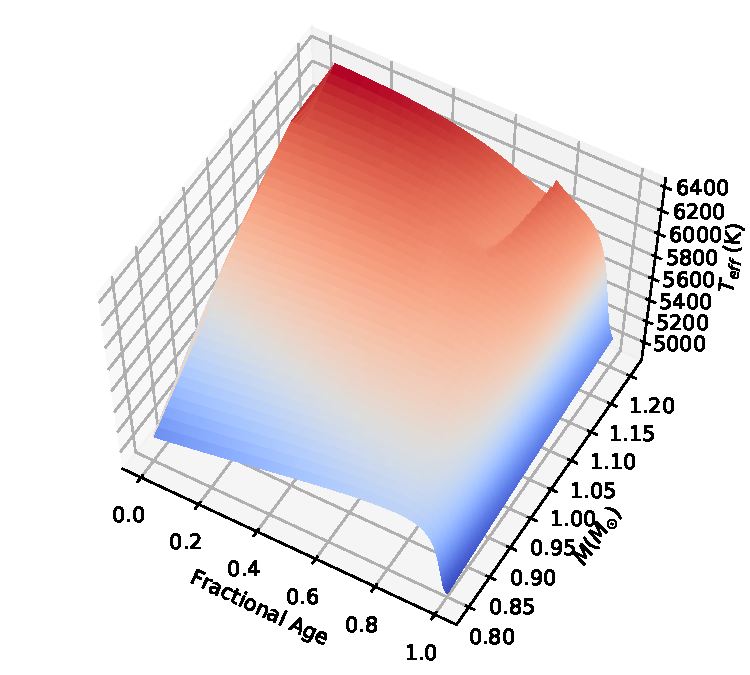
\includegraphics[width=1.\columnwidth]{2d_fage_data.pdf}
	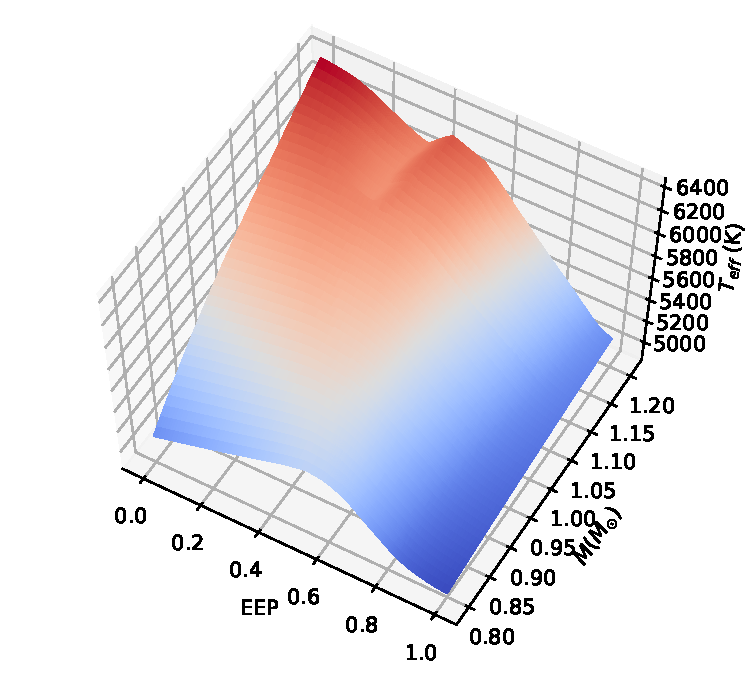
\includegraphics[width=1.\columnwidth]{2d_EEP_data.pdf}
     \caption{Surface plots of model effective temperature on the mass-fractional age (left) and mass-EEP (right) diagrams. Models in this figure are from the primary grid with fixed initial metallicity ($\rm [Fe/H]_{init}$ = 0.0), helium fraction ($Y_{\rm init}$ = 0.28) and mixing-length parameter ($\alpha_{\rm MLT}$ = 2.1). It can be seen that the effective temperature changes much smoother on the mass-EEP diagram at the blue hook and turn-off points.}
    \label{fig:eep}
\end{figure*}

\subsection{Sampling method}\label{sec:selection}

%We need three types of data for training, validating, and testing GP models. 
%
%Evolutionary tracks in the primary and additional grids are the training data. Off-grid tracks are divided 50-to-50 as validating and testing data . 
%Note that validating and testing datasets are not on the same evolutionary tracks so they are independent to each other. 
%Validating dataset is for validating the GP model in the training process and is mainly used for early stopping, which is a form of regularisation for avoiding overfitting. We choose off-grid models but not on-grid models as validating data because the grid is equally spaced. Without additional information between grid points, an optimiser could either use a smooth function or a periodic function to fit the data and find no obvious differences in the likelihood. We describe how we use validating data in Section \ref{sec:training}. Lastly, testing dataset is independent on the training process and used for evaluating the final GP models. 
There is a limitation of the data size in the GP framework, because the computational and memory complexity exponentially increase with the number of data points. In practice, the typical data size is on an order of $10^{4}$. Given that the grid contents $\sim 10,000,000$ stellar models, only a small subset can be used for training. The sampling method is hence important.
%
 A flat sampling is not appropriate, because the evolving step is not uniform at different evolutionary stages due to the \textsc{MESA} step-control strategy. For instance, stellar models are dense at the main-sequence and lower RGB but quite sparse at the subgiant stage. We test a few methods and find that using the displacement ($\delta d_{n}$) defined in Eq.~\ref{eq:disp} as the weight to sample models on an evolutionary track gives a relatively uniform data distribution at different evolutionary stages. 
%meets the above two requirements. 
%Firstly, we want the data to uniformly cover the parameter space for the best efficiency. Secondly, we need to highly weight models at phases where sharp changes present, e.g., models around the hook and turn-off points.   



